%% OJEPN article template for LaTeX
%% Licence: Creative Commons Attribution Share-Alike 4.0
%% Author:  Andy J. Wills
%% Adapted from a Creative Commons template by Jonathan Baron

\documentclass[twocolumn]{article}
\usepackage[utf8]{inputenc}
\usepackage[T1]{fontenc}
\usepackage[english]{babel}
\usepackage{ifpdf,amsmath,amsthm,amssymb,amsfonts,newtxtext,newtxmath} 
\usepackage{array,graphicx,dcolumn,multirow,hevea,abstract,hanging}
\usepackage[labelfont=sc,textfont=sf]{caption}
\usepackage[hyperfootnotes=false,breaklinks=true]{hyperref} % was dvipdfmx
\urlstyle{rm}
\usepackage[hyphenbreaks]{breakurl}
%\usepackage{natbib} % must come afer hyperfootnotes
%\setlength{\bibsep}{0pt}
\usepackage{booktabs} % \toprule \midrule \bottomrule \cmidrule(lr){a-b}
% define centered and ragged columns:
\newcolumntype{L}[1]{>{\raggedright\arraybackslash }p{#1}} % can use m{}
\newcolumntype{C}[1]{>{\centering\arraybackslash }p{#1}}
\newcolumntype{R}[1]{>{\raggedleft\arraybackslash }p{#1}}
\newcolumntype{d}[1]{D{.}{.}{#1}} % d{3.2} for 3 places on l, 2 on r
\newcommand{\mc}{\multicolumn}
\topmargin=-.3in \oddsidemargin=-.1in \evensidemargin=-.1in \textheight=9in \textwidth=6.8in
\setlength\tabcolsep{1mm}
\setlength\columnsep{5mm}
\setlength\abovecaptionskip{1ex}
\setlength\belowcaptionskip{.5ex}
\setlength\belowbottomsep{.3ex}
\setlength\lightrulewidth{.04em}
\renewcommand\arraystretch{1.2}
\renewcommand{\topfraction}{1}
\renewcommand{\textfraction}{0}
\renewcommand{\floatpagefraction}{.9}
% \renewcommand{\baselinestretch}{1.00} \large\normalsize % for fixing spaces
\widowpenalty=1000
\clubpenalty=1000
\setlength{\parskip}{0ex}
\let\tempone\itemize
\let\temptwo\enditemize
\let\tempthree\enumerate
\let\tempfour\endenumerate
\renewenvironment{itemize}{\tempone\setlength{\itemsep}{0pt}}{\temptwo}
\renewenvironment{enumerate}{\tempthree\setlength{\itemsep}{0pt}}{\tempfour}

%%%%%%%%%%%%%%%%%%%%%%%%%%%%%%%%%%%%%%%%%%%%%%%%%%%%%%%%%%%%%%%%%%%%%
\setcounter{page}{1} % start with first page

\title{How to use this template}

\author{
Andy J. Wills\thanks{School of Psychology, Plymouth University, U.K. Email: andy@willslab.co.uk}\;\,\thanks{Some other address.}
\and 
  Some O. Person\thanks{Yet another place.} 
\and
  Y. Another Author\footnotemark[2] % indicates same as 2nd thanks
}


\date{} % leave empty
\begin{document} % goes here

% fill in short title
\newcommand{\jref}{https://wwww.ojepn.com/vol1.html}
\newcommand{\jhead}{Open Journal of Experimental Psychology and Neuroscience, Vol.~1,}
\newcommand{\jdate}{January 2020}
\pagestyle{myheadings} \markright{\protect\small \href{\jref}{\jhead}, \jdate \hfill SHORT TITLE \qquad}
\begin{htmlonly}
\href{\jref}{\jhead}, \jdate, pp.\
\end{htmlonly}
%\begin{latexonly}
\twocolumn[
\vspace{-.3in}
{\small \href{\jref}{\jhead}, \jdate, pp.\ XXX--XXX}
%\end{latexonly}

\maketitle

%\begin{latexonly}
\vspace{-3mm}
\begin{onecolabstract}
%\end{latexonly}
The abstract is a brief (usually one paragraph) summary
of the whole paper, including the problem, the method for solving
it (when not obvious), the results, and the conclusions suggested
or drawn.  The reader should not have to read
any of the rest of the paper in order to understand the abstract
fully.  Many readers will read only the abstract.  Other readers
will use it to decide what to look for in the paper, or to decide
whether to read the whole thing. 

\smallskip
\noindent
Keywords: journal, template, latex
%\begin{latexonly}
\end{onecolabstract}\bigskip
]
%\end{latexonly}

{\renewcommand{\thefootnote}{}
\footnotetext{ % note blank lines above and below acknowledgment

  We acknowledge our funders and tech support.

Copyright: \copyright\ 2019.
The authors license this article under the terms of the
\href{http://creativecommons.org/licenses/by/3.0/}{Creative Commons
  Attribution Share-Alike 4.0 License.}
}}

\saythanks

\setlength{\baselineskip}{12pt plus.2pt}

\section{Introduction}

Here is some meaningless text as an example. Delete all the text that is not part of your paper.

Einstein said that $E = MC^2$. Many authors (Jones, 2016; Smith, 2017) have trouble replicating this result. Our hypothesis is that $E = MC^3$.

\section{Method} % example of a heading

Table 1 is an example of a one-column table using new column definitions.

%Table 1
\begin{table}[t]
\caption{Experiment 3: Mean (SD) willingness to contribute to identified
and unidentified victims, for self and for the average student.}
\begin{tabular}{L{.7in}C{.7in}C{.7in}C{.7in}}\toprule
 & Self & Average student & Total\\\midrule
Identified victim & 68.28 (55.77) & 45.30 (66.17) & 56.79 (61.89)\\
Unidentified victim & 54.06 (61.89) & 38.63 (67.20) & 46.35 (60.63)\\\midrule
Total & 61.17 (58.81) & 41.97 (66.51) & \\\bottomrule
\mc{4}{p{2.8in}}{Here is a meaningless note about this table.}\\
\end{tabular}
\end{table}

Use ``table*'' with the asterisk when the table needs 2
columns.  A table will generally go at the top of the first page that
refers to it, or as soon after that pages as possible. Do not assume
that tables will appear at the place they are put in the text. In the
tex file, they generally have to go before they are mentioned, in
order to appear in the best place.\footnote{Footnotes at the end of
  sentences should go after the period.}

\section{Results}

Use subsections and subsubsections etc. freely.

Figure 1 is an example of a one-column figure. 

\begin{figure}[t!]
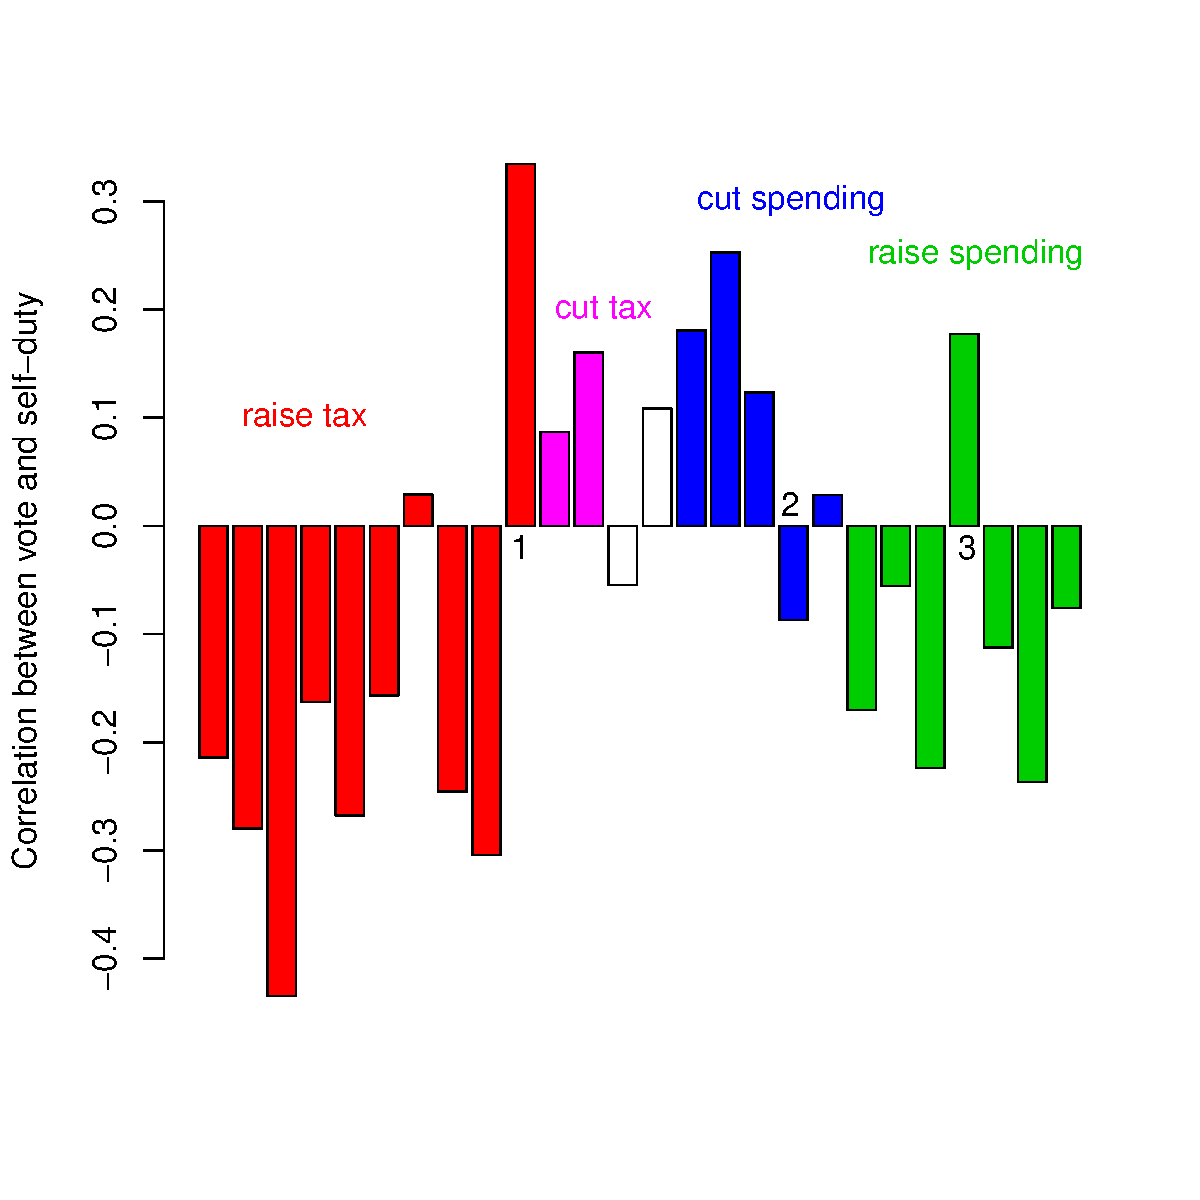
\includegraphics[width=\columnwidth]{dut11.pdf}
\caption{The caption goes under the figure like this. Note that
  columnwidth is the width of a column. But you can use any units,
  e.g., ``3in'' or ``50mm''.}
\end{figure}

Figure 2 is a two-column figure. A figure will generally go at the top of
the first page that refers to it, or as soon after that page as
possible. Do not assume that figures will appear at the place they are
put in the text. In the tex file, they generally have to go before
they are mentioned, in order to appear in the best place.

\begin{figure*}[t!]\centering
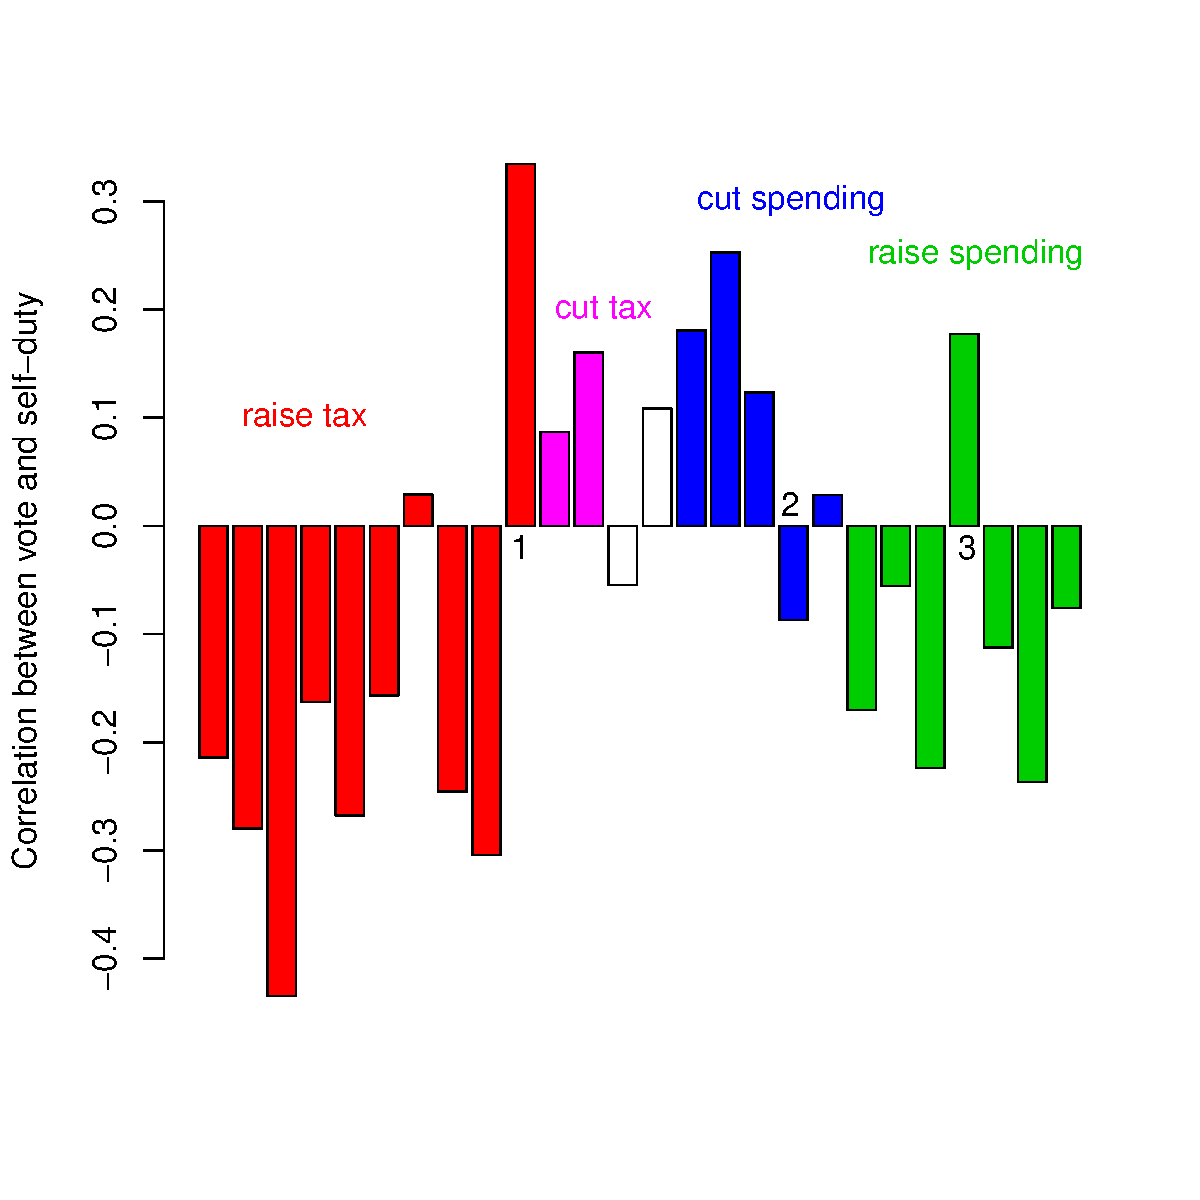
\includegraphics[width=5in]{dut11.pdf}
\caption{The caption like this.}
\end{figure*}

\section{Discussion}

It turns out that $E = MC^2$.  Specifically,
\begin{equation}
E = \frac { \sum_{i=1}^n ( M_i C )^2 }{ \alpha + \beta }
\end{equation}
Equation 1 is true.

In order to pad things out a bit, here's the opening of ``A Christmas Carol'' by Charles Dickens, from Project Gutenburg.

MARLEY was dead: to begin with. There is no doubt
whatever about that. The register of his burial was
signed by the clergyman, the clerk, the undertaker,
and the chief mourner. Scrooge signed it: and
Scrooge's name was good upon 'Change, for anything he
chose to put his hand to. Old Marley was as dead as a
door-nail.

Mind! I don't mean to say that I know, of my
own knowledge, what there is particularly dead about
a door-nail. I might have been inclined, myself, to
regard a coffin-nail as the deadest piece of ironmongery
in the trade. But the wisdom of our ancestors
is in the simile; and my unhallowed hands
shall not disturb it, or the Country's done for. You
will therefore permit me to repeat, emphatically, that
Marley was as dead as a door-nail.

Scrooge knew he was dead? Of course he did.
How could it be otherwise? Scrooge and he were
partners for I don't know how many years. Scrooge
was his sole executor, his sole administrator, his sole
assign, his sole residuary legatee, his sole friend, and
sole mourner. And even Scrooge was not so dreadfully
cut up by the sad event, but that he was an excellent
man of business on the very day of the funeral,
and solemnised it with an undoubted bargain.

The mention of Marley's funeral brings me back to
the point I started from. There is no doubt that Marley
was dead. This must be distinctly understood, or
nothing wonderful can come of the story I am going
to relate. If we were not perfectly convinced that
Hamlet's Father died before the play began, there
would be nothing more remarkable in his taking a
stroll at night, in an easterly wind, upon his own ramparts,
than there would be in any other middle-aged
gentleman rashly turning out after dark in a breezy
spot--say Saint Paul's Churchyard for instance--
literally to astonish his son's weak mind.

Scrooge never painted out Old Marley's name.
There it stood, years afterwards, above the warehouse
door: Scrooge and Marley. The firm was known as
Scrooge and Marley. Sometimes people new to the
business called Scrooge Scrooge, and sometimes Marley,
but he answered to both names. It was all the
same to him.

Oh! But he was a tight-fisted hand at the grind-stone,
Scrooge! a squeezing, wrenching, grasping, scraping,
clutching, covetous, old sinner! Hard and sharp as flint,
from which no steel had ever struck out generous fire;
secret, and self-contained, and solitary as an oyster. The
cold within him froze his old features, nipped his pointed
nose, shrivelled his cheek, stiffened his gait; made his
eyes red, his thin lips blue; and spoke out shrewdly in his
grating voice. A frosty rime was on his head, and on his
eyebrows, and his wiry chin. He carried his own low
temperature always about with him; he iced his office in
the dog-days; and didn't thaw it one degree at Christmas.

External heat and cold had little influence on
Scrooge. No warmth could warm, no wintry weather
chill him. No wind that blew was bitterer than he,
no falling snow was more intent upon its purpose, no
pelting rain less open to entreaty. Foul weather didn't
know where to have him. The heaviest rain, and
snow, and hail, and sleet, could boast of the advantage
over him in only one respect. They often "came down"
handsomely, and Scrooge never did.

Nobody ever stopped him in the street to say, with
gladsome looks, "My dear Scrooge, how are you?
When will you come to see me?" No beggars implored
him to bestow a trifle, no children asked him
what it was o'clock, no man or woman ever once in all
his life inquired the way to such and such a place, of
Scrooge. Even the blind men's dogs appeared to
know him; and when they saw him coming on, would
tug their owners into doorways and up courts; and
then would wag their tails as though they said, "No
eye at all is better than an evil eye, dark master!"

But what did Scrooge care! It was the very thing
he liked. To edge his way along the crowded paths
of life, warning all human sympathy to keep its distance,
was what the knowing ones call "nuts" to Scrooge.


Once upon a time--of all the good days in the year,
on Christmas Eve--old Scrooge sat busy in his
counting-house. It was cold, bleak, biting weather: foggy
withal: and he could hear the people in the court outside,
go wheezing up and down, beating their hands
upon their breasts, and stamping their feet upon the
pavement stones to warm them. The city clocks had
only just gone three, but it was quite dark already--
it had not been light all day--and candles were flaring
in the windows of the neighbouring offices, like
ruddy smears upon the palpable brown air. The fog
came pouring in at every chink and keyhole, and was
so dense without, that although the court was of the
narrowest, the houses opposite were mere phantoms.
To see the dingy cloud come drooping down, obscuring
everything, one might have thought that Nature
lived hard by, and was brewing on a large scale.


\subsection{How to add Lists}

You can make lists with automatic numbering \dots

\begin{enumerate}
\item Like this,
\item and like this.
\end{enumerate}
\dots or bullet points \dots
\begin{itemize}
\item Like this,
\item and like this.
\end{itemize}

References should be in APA style. Examples are below.


\section*{References}

\begin{hangparas}{1em}{1}

  Aarts, H., \& Dijksterhuis, A. (1999).  How often did I do it?
  Experienced ease of retrieval and frequency estimates of past
  behavior.  \textit{Acta Psychologica, 103}(3), 77--89. \url{http://someurl.html}.

  Barberis, N. \& Thaler, R. (2003). A survey of behavioral finance.
  In G. M. Constantinides, M. Harris \& R. Stultz (Eds.),
  \textit{Handbook of the Economics of Finance,} pp.\ 1053--1123.
  Elsevier Science, North Holland, Amsterdam

Grice, H. P. (1975).  Logic and conversation. In P. Cole \& J.
L. Morgan, (Eds.), \textit{Speech Acts}, pp.\ 41--58. London: Academic
Press. \url{http://dx.doi.org/3.14159--1x}.
\end{hangparas}

\bigskip

\section*{Appendix}

The asterisk means that these divisions are not numbered.

\subsection*{How to create Sections and Subsections}

Use section and subsections to organize your document. We'll handle all the formatting and numbering automatically.

\end{document}

%%% Local Variables:
%%% mode: latex
%%% TeX-master: t
%%% End:
